\documentclass[a4paper,12pt]{article}

\usepackage[utf8]{inputenc}
\usepackage[ngerman]{babel}
\usepackage[T1]{fontenc}
\usepackage{graphicx}
\usepackage[cache=false]{minted}
\usepackage{dirtree}
\usepackage{biblatex}
\usepackage[strings]{underscore}
\addbibresource{literatur.bib}



\begin{document}
\begin{titlepage}
    \begin{center}
        \vspace*{1cm}
        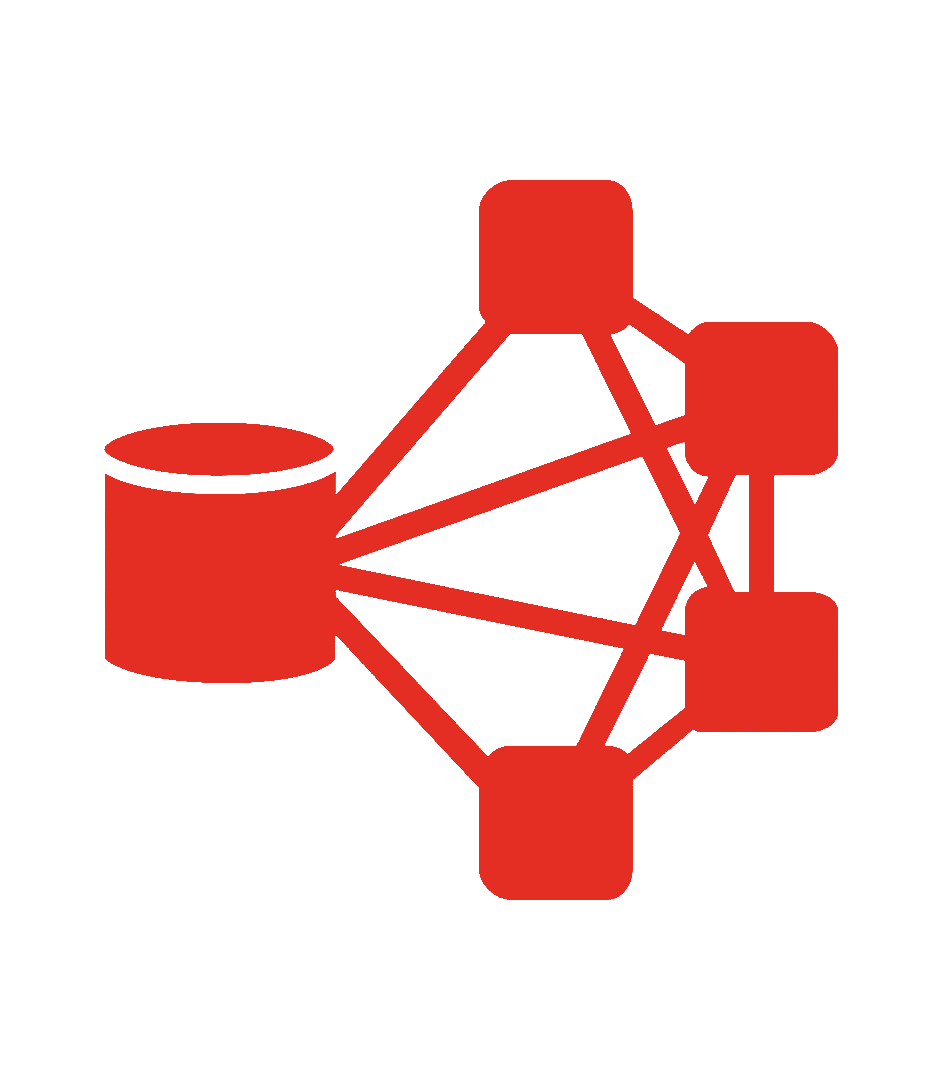
\includegraphics[width=10cm]{Logo.png}
        
        \textbf{\huge MapReduce-System}
        
        \vspace{0.5cm}
        NVS Projekt 2
                 
        \vspace{1.0cm}
    
        \textbf{Alexander Grill 5CHIF}
        
        \today
        
        \vfill
                 
                 
        \vspace{0.5cm}
                 
        Informatik\\
        HTBLUvA Wr.Neustadt\\
        Österreich\\

                 
    \end{center}
\end{titlepage}  
\newpage
\tableofcontents
\newpage


\section{Einführung}
In diesem Kapitel werden die Gründe der Umsetzung und das Thema, worum es in dieser Arbeit geht, genau erläuter. Es wird auch
darauf eingegangen, welche Thematiken das Projekt umfassen soll und wie sich die Benotung auseinander setzt.

\subsection{Vorwort}
Der Virus "COVID-19" war im Jahr 2020 für die gesamte Bevölkerung auf der Erde eine rießengroße Herausforderung. Die Situation änderte sich am Begin im daruffolgendem Jahr 2021 nicht, 
deshalb beschloss die Bundesregierung weiter Maßnahmen, Ausgangsbeschränkunge, Grenzkontrollen, FFP2-Maskenpflicht und weitere Regeln die, die Bevölkerung einzuhalten hat. Alle Schüler in Österreich müssen die Schule 
blockweiße besuchen. Nur mit einem davor verpflichtetenden Schnelltest und FFP2-Maske dürfen sie die Schule betrehten. Da die Projektarbeiten im ersten Semster dementsprechend gut ausgefallen sind, beschloss Herr Professor 
Kolousek, dass Schüler in den fünften Klassen im Fach NVS statt der Praktischen Arbeit und dem Theorie Test eine Projektarbeit über den Semsterstoff machen müssen. Folgendessen muss die Dokumentation, über das gewählte Thema, dementsprechend einen
weiteren Umfang umfassen als beim ersten Projekt im ersten Semster. Im praktischen Teil geht es in diesem Projekt, darum ein Map-Reduce System in Kombination mit Server-Client Kommunikation zu implementier. Im theoretischen Teil, werden die Grundlagen die für die 
Umsetzung relevant sind erklärt. Zusätzlich beinhaltet dies auch sämtliche Abschnitte wie, die Source Code Dokumentation, Abläufe, Erklärung bezgl. MapReduce-System, Aufbau und Anwendungsfälle.
\begin{description}
    \item[Die zu erreichende Note hängt prinzipiell von der] ~\par
    \begin{itemize}
        \item Beispielkategorie
        \item Art der Kommunikation
        \item Funktion, Umfang und Tiefe der Implementierung
        \item Fehlerbehandlung
        \item Ausgaben, Einhaltung der Coding Conventions, Kommentare
        \item Repository: Commits, Issues
        \item Ausarbeitung
        \item Einhaltung der Richtlinien
      
    \end{itemize} 
\end{description}
\subsection{Motivation}
In diesem NVS Projekt geht es darum, ein MapReduce-System mit der Programmiersprache C++ unter Linux mittels g++ Compilier umzusetzten.
Im kurzem zusammengefasst soll eine große Menge an komplexen, unstrukturierten und eine Art von aufwendigen Daten verarbeitet werden. 
Das heißt es sollen Daten, die planlos abgespeichert sind, zusammengefasst werden, sodass diese wieder ihren Nutzen oder Sinn erbringen. Diese können
dann für weiter Verarbeitungsschritte oder Datenanalysen verwendet werden. Die Daten werden am Beginn in kleiner Packete aufgeteilt und diese werden identifiziert mit einem eindeutigen
Schlüssel. In der nächste Phase werden die einzelnen Packete parallel von unterschiedlichen, getrennten und unabhängigen Prozesse zusammengefasst. Danach werden die gruppierten Daten wieder 
einen Schlüssel zugeordnet, sodass diese wieder zusammengefasst und minimiert werden. Die Kommunikation zwischen den einzelnen Knoten, soll in dieser Arbeit mittel Server-Client Kommunikation passiern.
Der Server hört auch einem Port ab, ob sich ein Client damit verbinen möchte, wenn eine Verbindung aufgebaut werden kann, soll die Splittung der Daten passier, daraufhin soll das Resultat weiter an dem Server gegeben werden, bis 
alle Daten vereint auf dem Master Server liegen. Die bearbeitetn Daten werden schlussendlich in einem JSON-File abgespeichert.
\section{Aufgabenstelllung}
Diese Kapitel umfasst die genaue Erläuterung der Aufgabenstelllung, als auch die Themenbereiche die dieser Projektarbeit. Darüber hinaus wird auch über die Idee der Umsetzung geschrieben.

\subsection{Erläuterung der Aufgabenstellung}
Ziel ist es das eine Menge von unstrukturierten Daten, so verarbeitet werden, dass diese danach wieder in ordnungsgemäßer Struktur vorliegen. Zuerste müssen die Daten aufgeteilt werden. Sie werden in einer Key-Value Form abgepeichert, somit kann
der Value, also der abgespeicherte Datensatz, mittels Key eindeutig identifiziert werden. Nachdem die Daten zusammengefasst vorliegen, werden sie in nächste Schritt auf einzelne Knoten aufgeteilt. Diese erlangen von den einzelenen Clients die Daten in Key-Value Form und fassen diese wieder zusammen, bis die Daten zu einem Master Knoten ankommen und dort schlussendlich in geordneter Form darliegen.
Die Aktionen, der Datenverarbeitung verläuft ständig unter paralleler Abfolge, die Aufgaben werden aufgeteilt und gleichlaufen auf verscheidenen Knoten aufgeteilt.

\subsection{Idee}
Das Projekt ist so aufgebaut, das es acht oder mehr Clients gibt, zwei Slave Server und einen Master Server. Ein Benutzer(Client) kann einen beliebige Anzahl von Zeichenketten, die er dem Programm beim Aufruf mitübergibt, erzeugen und diese werden dann in einer Datei abgespeichert. Zuästzlich wird dem Benutzer auch angeboten dem Speichertort der Datei selbst auszuwählen. Nachdem die ungeordneten Daten in einer Datei 
abspeichert sind, beginnt die nächste Phase des Map-Reduce System. Die Datei wird zeilenweise durchgegangen. Die Zeichenketten werden in einem Art Dictionary als Key-Value Form abspeichert, daduch kann jeder eingefügte Datensatz identifiziert werden. Wenn der Datensatz in diesem Dictionary schon existiert, dann wird der Value, der als Counter festlegt wie oft die Zeichenfolge im Text vorkommt, um eins erhöht. Nachdem kompletten Durchlauf der Datei sind alle Daten
in diesem Dictionary abspeichert. Dadurch, dass mehrere Clients das System zum gleichen Zeitpunkt unabhängig voneinander nutzen können, wird das durchforsten der Datei von anderen Prozessen nicht beeinflusst. Nachdem ein Prozess mit der Datenabspeicherung fertig ist, sendet er die Daten an den jeweiligen Slave Server der zu diesem Zeitpunkt nicht beschäftigt ist. Wenn der Server von einer gewissen Anzahl von Clients die Daten bekommt, beginnt er danach mit der Map Phase. An dieser Stelle werden
die gesendetet Daten wieder per Key zusammengefasst und strukturiert. Die Abarbeitung erfolgt auch in diesem Fall parallel zu einem weiter Slave Knoten, der die selbe Art und Weise der Datenverarbeitung nutzt. Schlussendlich wird das Result an den Master Server geschickt. Letzendlich bringt dieser all seine empfangen Daten in eine Struktur, die im Nachhinein für Datenanalysen eingesetzt werden können.
\subsection{Themenbereiche}
\begin{description}
    \item[Diese Arbeit umfasst folgende Thematiken] ~\par
    \begin{itemize}
        \item Grundlagen und Basiskonzepte, Nachrichtenübertragung, Netzarchitektur
        \item Internetprotokoll
        \item Transportprotokolle
        \item Prozesse und Threads
        \item Synchronisation und parallele Programmierung
        \item Kommunikation, Serverprogrammierung, verteilte Systeme
        \item TCP/IP Programmierung      
    \end{itemize} 
\end{description}
\newpage
\section{Grundlagen}

\subsection{Was ist ein MapReduce System?}
Das Verfahren wurde 2004 von Google entwickelt für die Indexierung von Webseiten. Das Framework wird bei Datenbanken eingesetzt und dient zur Verarbeitung von großen, komplexen, unstrukturierte Datenmengen.
Dieses Verfahren findet Anwendung für BigData und Datawarehouse, weil in solchen Fällen große Datenmengen in kürzester Zeit mittels Software verarbeitet, analysiert, aggregiert als auch kompremiert werden. 
Map Reduce parallelisiert die Bearbeitung, durch die Verteilung auf mehrere gleichzeitig auszuführende Tasks. Der Grund, warum dieses Framework solche Datenmengen verarbeiten kann ist, weil die Aufgaben auf mehreren Rechnern aufgeteilt werden. Jeder einzelne Rechner startet Prozesse, die Parallel die Daten verarbeitet und auswertet.
Ein einzelner Rechner stoßt schnell an seine Grenzen, deshalb ist die Verarbeitung von Daten, mittels mehreren Knoten sehr effizient und bietet eine bessere Performance.
Das Verfahren wurde in vielen verschiedenen Verfahren eingesetzt wie zum Beispiel für die Indizierung von Webseiten, nach einer Suchanfrage mit beliebigen Zeichenketten, ebenso im Umfeld von Google News wird MapReduce verwendet. Andere große Internetfirmen wie Yahoo, die ebenfalls das Verfahren für die Indexierung von Webseiten verwenden, 
als auch Facebook verwendet das System, um Spam Messages zu minimierung und die Ads zu optimieren. Wohingegen Amazon das Verfahren für das Clustering der Produket verwendet

\subsection{Map und Reduce}
Die beiden Grundfunktionen des Verfahrens sind Map und Reduce. Sie sorgen für die Aufteilung der Aufgaben in kleinere parallelisierten Arbeitspakete und führen am Ende die Ergebnisse zusammen. Bei großen relationalen Datenbanken und komplexen Queries lassen sich typische Problem, bezglüch Verarbeitung von großen Datenmengen beseitigen.
Die Map Funktion, verteilt die Aufgaben an unterschiedlichen Knoten eines Clusters. Die Reduce Funktion sortier die verfassten Ergebnisse und fügt sie am Ende wieder zusammen.
Die Funktionen Map und Reduce werden vom User bereitgestellt, weil diese schließlich zu den bereitgestellten Daten passen müssen.
\cite{mrsystem}
\newpage

\subsection{Ablauf}

\begin{figure}[h]
    \centering
    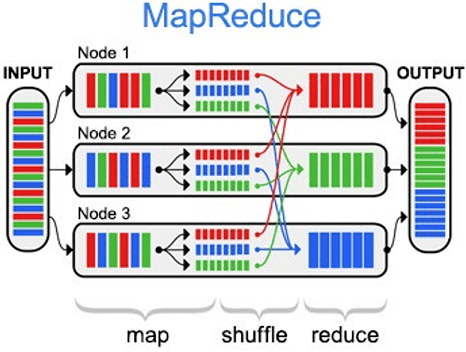
\includegraphics[width=6.1cm]{mapreduce.png}
\end{figure}
\begin{description}
    \item[Das Verfahren verläuft durch folgende Schritte:] ~\par
    \begin{itemize}
        \item Split
        \begin{itemize}
            \item{Die bereitgestellten Daten werden aufgeteilt. Jeder Datensatz darin ist identifiziert durch
            einen Schlüssel-Wert. Diese Datenmenge wird nun in kleinere Datenmengen aufgeteilt
            und vom Master an die verfügbaren Knoten verteilt.}
        \end{itemize}
        \item Map 
        \begin{itemize}
            \item{Nun wendet jeder Knoten auf die Daten die Map-Funktion an, die schließlich Key/Value Paare zurückgibt. Diese Ergebnisse werden zwischengespeichert.}
        \end{itemize}
        \item Shuffel
        \begin{itemize}
            \item{Bei diesem Schritt geht es darum den reduce-Knoten, die entsprechenden Daten zuzuteilen.
            Diese Zuteilung entspricht einer Fragmentierung.
            Hierbei wird den Knoten, die reduce ausführen, ein Key zugeteilt. Diese Knoten holen sich
            dann die bereits durch Map entstandenen Datensätze mit diesem Key und wenden reduce an.}
        \end{itemize}
        \item Reduce
        \begin{itemize}
            \item{Grundsätzlich ist die Aufgabe dieser Funktion, die Key/Value Paare anhand des Schlüssels
            zusammenzufassen und dabei die Summe der einzelnen Values zu bilden. Demnach ist die
            Ausgabe der Reduce-Funktion wieder ein Key/Value Paar mit dem gleichen Aufbau wie vor
            der Verarbeitung.
            Dies ermöglicht es, dass reduce mehrere Male angewendet werden kann, bis schließlich alle
            Daten gesammelt wurden.}
        \end{itemize}
    \end{itemize} 
\end{description}

\subsection{Vorteile Nachteile eines Map-Reduce Systems}
Map Reduce bietet eine Menge an Vorteilen, gegenüber den klassischen Verfahren der Datenverarbeitung, wie
sie in den relationalen Datenbanksystemen verwendet werden. \\ \\
Ein wesentlicher Vorteil ist, dass für die
Verwendung eines solchen System ein einfacher normaler Rechner benötigt wird und keine Highend-Server. Ein Cluster-Verbund für die parallelisiert
Datenverarbeitung kann bei Notwendigkeit ohne großen Aufwand realisiert werden. Ein Cluster-Verbund ist ein Netzwerk, das aus mehreren Rechner besteht die gleichzeit miteinander verbunden sind 
und sich Daten austauschen. Aus diesem Grund ist ein MapReduces-System sehr kostensparsam und kann mit wenig Know-How und Erfahrungen umgesetzt und
schlussendlich in Verwendung gebracht werden. \\ \\
Ein weiterer Vorteil ist auch die Skalierbarkeit. Da die Daten auf den jeweiligen Knoten
aufgeteilt werden, bietet das System eine zuverlässige Ausfallstoleranz und Verfügbarkeit, denn wenn ein Knoten ausfallen sollte, werden die Daten einfach an einem
anderen Knoten und dort verarbeitet, somit läuft das System zu jederzeit in einem stabilen Zustand. \\ \\
Durch die parallelisierte Verarbeitung von Daten ist dieses Verfahren deutlich effizienter und perfomanter als die Datenverarbeitung
in relationalen Datenbanken. Im Terabyte-Bereich dauert das Verfahren oft nur Minuten, im Petabyte-Bereich Stunden, wobei andere Systeme deutlich mehr Zeit und Ressourcen für die Verarbeitung
benötigen.\\ \\
Während die Berechnungen schnell gehen, dauert der Datenzugriff länger als bei anderen Methoden. 
Die Daten müssen erst über das Netzwerk gestreamt werden. Dabei ist die Netzanbindung der Flaschenhals, vor allem im Hinblick auf die sehr unterschiedlichen Rechner innerhalb des Clusters und deren unterschiedliche schnelle Netzanbindung.\\ \\
Um die Geschwindigkeit zu erhöhen, kann ein Cluster ausschließlich aus High-End-Servern bestehen. In diesem Fall sind die Kosten für das MapReduce-Verfahren immens hoch.
\cite{vorteil/nachteilemrsystem}
\newpage
\noindent
\subsection{Parallel Programming}
Unter Parallel Programming versteht man die Aufteilung einer Problemstellung in weitere kleinere Teilprobleme die nebenläufig abgearbeitet werden, dabei wird jedes Teilproblem einzelnt gelöst und dadurch auch das Gesamtproblem effizient und schnell gelöst werden. 
\\Dabei kann die Problemstellung schneller gelöst werden, weil die Abarbeitung aufgeteilt wird und die Teilprobleme unabhängig voneinander gleichzeitig bearbeitet werden können. Parallel Programming wird heutezutage in Branchen wie Chemie, Biologie, Medizin, Maschinenbau, Baustatik, Simulationen, Suchen in großen Datenbestände etc. angewendet.\\\\
\textbf{Mooresches Gesetz\\}
"Die Anzahl der Transistoren pro Chip verdoppelt sich etwa alle zwei Jahre". Das heißt je mehr Transistoren sich auf einem Chip befinden, desto mehr Funktionalität kann parallel abgearbeitet werden.Laut der Webseite "nature.com" wird die Halbleiterindustrie im März 2016 anerkennen, dass Moore's Law nicht mehr eingehalten werden kann. Demnach werden Chips nicht mehr zwangsläufig schneller, aber Fortschritt und Effizienzmaximierung wird es weiterhin geben.\\\\
\textbf{Wirth´sches Gesetz\\}
"Die Software wird schneller langsamer, als die Hardware schneller", darunter versteht man, dass die Anforderungen an die Software immer aufwendiger, größer und komplexer wird und die Hardware diese Softwaren sehr langsam bis gar nicht verarbeiten können.\\\\
\textbf{Taktfrequenzen\\}
Die Taktfrequenze verdoppelte sich in den 1990-er Jahre alle 18 bis 20 Monaten, aber seit 2000 bis 2005 ist das nicht mehr der Fall. Heute finden maximial 4GHz im Desktop und Serverbereich Anwendung.\\Man spricht von einer sogenannten "Frequency Wall", wenn die Taktfrequenz nicht mehr erhöt werden kann, weil höhere Frequenz bedeutet höhere Spannung, höhere Spannung heißt, höhere Verlustleistung. Das hat zur Folge, dass die entstehnde Wärme, die durch den Anhib der Taktfrequenz und durch die Datenverarbeitung entsteht, nicht mehr abgeführt werden kann.
Existierende nicht parallelisierte Software profitiert nicht mehr automatisch von der Leistungsseigerung der Hardware. Ein weiterer Nachteil ist, dass das Laufzeitverhalten paralleler Algorithmen schwieriger nachvollziehbar sein kann als das eines äquivalenten sequentiellen Algorithmus.\\\\
\textbf{Lösungsansätze\\}
Der einfachste Lösungsantz ist der, indem man dein Problemraum einschränkt, damit ist gemeint der Algorithmus wird für den jeweiligen Aufwand eingeschränkt und angepasst. Eine weiter Idee wäre, dass man den Algorithmus selbst optimiert, jedoch ist das nicht immer möglich. Weiters ist die Verbesserung der Implementierung von Vorteil.(z.B Facebook -> eigener String)
Auch durch den Bereich Hardware kann eine Software verbessert werden, dennoch ist diese Strategie mit hohen Kosten verbunden. Am effizientesten ist es hingegen, die Software in Teilprobleme aufzuteilen und diese parallel abzuarbeiten. Da ein Prozessor mehrere Kerne besitzt können mehrere unterschiedliche unabhängigvoneinandere Prozesse abgearbeitet werden. 
\begin{description}
    \item[Möglichkeiten der Parallelisierung] ~\par
    \begin{itemize}
        \item Zerlegung der Gesamtaufgabe in kleinere, mehreren Teilaufgaben, sodass die maximale Auslastung aller Prozesser(HW) stattfindetn, weil jede Teilaufgabe auf einem einzelnen Prozessor stattfindet.
        \item Zerlegung der Gesamtaufgabe in kleinere, mehreren Teilaufgaben, die hintereinander ausgeführt werden, allerding wird die Gesamtzeit der Lösung einer Gesamtaufgabe nich kürzer und der Durchsatz bei der Lösung von vielen Aufgaben höher.
        \item Zerlegung der Gesamtaufgabe in kleinere, mehreren Teilaufgaben, die hintereinander ausgeführt werden, aber mit spezieller Hardware gelöst werden.
    \end{itemize} 
\end{description}
\textbf{Pipelinig\\}
Pipelinig beschreibt den Vorgang wie ein Prozessor vorgeht, wenn er mehrere Befehle verarbeiten werden müssen. Als Erstets wird der Befehl aus dem Arbeispeicher geladen(fetch), weiters wird dieser Befehlt in Maschiensprache umgewandelt und dekodiert(decode), werden zusätzliche Daten benötigt läd der Prozessor diese aus Registern oder aus dem Arbeitspeicher. Folgedessen wird der Befehlt schlussendlich ausgeführt(execute) und das Resultat des Befehls wird in einem Register oder im Arbeitspeicher geschrieben(write back).
Die einzelnen Schritte werden in einer eigenen Hardwarekomponente ausgeführt, deshalb ist es möglich, wenn ein Befehl gefechte wird und danach dekodiert werden kann, kann in der Zeit, in der er dekodiert wird, ein andere Befehl gefetched werden. Das ist möglich bei jedem einzelnen Schritt.
\cite{parallelprogramming}

\subsection{Kommunikation}
Das Prinzip der Kommunikation im Internet ist, dass man strikt sein sollen beim Senden der Daten und tolerant beim Empfängen. Der Zweck einer Kommunikation sind die Interoperabilität, das bedeutet
das mehrere Systeme die aus Rechner bestehen in der Lage sind Daten untereinander auszutauschen, und die Fehlertolaranz, das bedeutet das die Daten durch festegelegte Regeln übertragen werden aber beim Empfangen in einer
gewünschen Form umgewandelt werden können.

\begin{description}
    \item[Beziehungen zwischen den einzelnen Knoten] ~\par
    \begin{itemize}
        \item one-to-one
        \begin{itemize}
            \item{Ein Knote kommuniziert mit einen anderen Knoten}
        \end{itemize}
        \item one-to-many
        \begin{itemize}
            \item{Ein Knoten spricht mit mehreren Knoten und alle lauschen und hören zu. Diese Art von Kommunikation zwischen den Rechner nennt man multicast}
        \end{itemize}
        \item one-to-any
        \begin{itemize}
            \item{Ein Knoten spricht mit mehreren Knoten, jedoch betrifft das nur einen Knoten von mehreren.}
        \end{itemize}
        \item many-to-one
        \begin{itemize}
            \item{Mehrere Knoten sprechen zu einen konkreten Knoten}
        \end{itemize}
        \item many-to-many
        \begin{itemize}
            \item{Mehrer Knoten kommuniziert mit mehreren anderen Knoten.\\}
        \end{itemize}
    \end{itemize} 
\end{description}
\textbf{Kommunikationsrichtung\\}
Beim Datenautausch ist wichtig festzuhalten, in welche Richtung die Daten übertragen werden. Mittel simplex werden die Daten nur in eine Richtung übertragen. 
Bei half-duplex werden die Daten ebenso in eine Richtung übertragen, jedoch kann die Richtung in der Übertragen wird änderen. Bei der Variante duplex werden die Daten in beide Richtungen übertragen wie im TCP Protokoll realisiert, werden zwei Streams
zur Verfügung gestellt um Daten zu senden und zu empfangen.\\\\\\\\
\textbf{Verbindungen\\}
Im Grunde genommen unterscheidet man zwischen verbindungsorientierter und verbindungsloser Kommunikation. Bei der verbindungsorientierter Kommunikation wird eine Verbindung zwischen zwei Knoten aufgebaut, danach werden Daten ausgetauscht und zum Schluss kommt es zur
Verbindungsabbau. Wohingegen bei der verbindungsloser Kommunikation nur die Datenübertragen werden und keine Verbindung aufgebaut und abgebaut wird. Es ist in der Regel effizienter, aber es wird nicht sichergestellt ob die Daten wirklich beim Empfänger angekommen sind.\\ \\
\textbf{Signalisierung\\}
Bei der Kommunikation werden auch Nachrichten ausgetauscht, die zum Aufbau, der Überwachung und dem Abbau einer Verbindug notwendig sind. Man spricht von in-bank signalling, es wird ein gleicher logischer Kanal wie Nutzdaten und Steuerungsdaten verwendet, oder out-of-band signalling, hier wird ein getrennter logischer Kanal verwendet. Es gibt einen
physischen Kanal der in mehrere logische Kanäle unterteilt sind. \\ \\
\textbf{Protokoll\\}
Für die Kommunikation benötigt man auch festgelegte Regeln, die für eine Kommunikation notwendig sind, darunter versteht man den Begriff Protokoll. Das betrifft das Format der Nachrichten, Reihenfolge der Nachrichten und die Spezifikation der Fehlersituation. Es gibt zustandsbehaftete und zustandlose Protokolle. zustandsbehaftete Protokolle sind, jene bei denen die Nachrichten
vom Zustand der zuvor gesendete Nachrichten abhängt. Bei dem zustandlos Protokol heißt, die Nachrichten sind unabhängig von zuvor gesendeten Nachrichten.\\\\
\textbf{Session\\}
Im Informationaustausch spielt auch der Begriff Session eine wichtige Rolle. Dieser beschreibt eine feste Beziehung zwischen kommunizierenden Prozessen mit vereinbarten Eigenschaften wie Namen, Ressourcen, Charakteristika. Dadurch bildet sich ein gemeinsamer Zustand zwischen dein einzelnen Prozessen. Um sicherzustellen welcher Knoten welcher ist und welche Rechte dieser hat 
bei der Kommunikation mit anderen hat, werden Mechanismen zu Authentifikation und Autorisierung. Bei HTTP sieht die Kommunikation folgendermaßen aus, ein Client der mittels Browser eine Seite aufruft sendet einen Request an den Server, dieser überprüft die Daten der Anfragen und welche Daten der Client benötigt und sendet den Client danach mittels Respone die angefragten Daten zurück.\\
Wird die Seite neu geladen so verschwinden auch die Daten die in einem Cache zwischengespeichert sind und für weitere Aktionen relevant sind. Dies kann oft zu Problem führen, deshalb wird ein sogenanter Session-Cookie verwendet, in dem Daten abgelegt werden, die in einer Session entstehen und für weitere Tätigkeiten relevant sind und in diesem abgespeichert werden.\\ \\
\textbf{Hierachie von Protokollen\\}
Protokolle sind hierachisch angeordnet, dass hat den Vorteil, dass mit Problemen zwischen den unterschiedlichen Protokollen besser umgehen kann und jede Schicht nur wissen muss was mit der darunterliegenden Schicht zu tun ist und wie Daten an die darüberliegenden Schicht geben kann. Die Schichten können auch ausgetauscht werden.
\\\\
\textbf{Kommunikationsstile\\}
Die Kommunikation kann durch unterschiedlichen Stillen durchgeführt werden wie zum Beipsiel wird ein gemeinsamer genutzer Knoten verwendet und auf diesem zugegriffen auf dem alle Daten abgespeichert werden, wie es bei Datenbanken der fall ist, beim Versenden von Nachrichten spricht man von nachrichten-orientierte Kommunikation. \\\\
Im Vergleich beim Aufruf einer Funktion oder Methoden die auf einem Client abgespeichert sind
spricht man von Entfernte Funktionsaufrufe (Entfernte Methodenaufrufe), wenn Daten verarbeite werden wenn sie eintreffen spricht man von stream-orientierter Kommunikation.\\\\
\textbf{synchron vs. asynchron\\}
Ein Nachrichtenautausch kann entweder synchron oder asynchron passierten. Bei einer synchronen Austausch wird die Operation begonnen, wenn der Sender die Nachricht initiert hat und der Empfänger bereit ist die Nachricht zu empfangen. Wobei bei einer asynchronen Nachrichtenaustauch, der Sender die Nachrichten unabhängig, ob der bereit ist oder nicht. 
\newpage
\begin{description}
    \item[Semantik der Nachrichtenübermittlung] ~\par
    \begin{itemize}
        \item no-wait-send
        \begin{itemize}
            \item{Der Sendeprozess wartet lediglich bis die Nachricht im Transportsystem zum Absenden bereitgestellt ist.}
        \end{itemize}
        \item synchronization send
        \begin{itemize}
            \item{Der Sendeprozess wartet bis die Nachricht vom Empfangsprozess entgegengenommen worden ist.}
        \end{itemize}
        \item remote-invocation send
        \begin{itemize}
            \item{Der Sendeprozess wartet bis die Nachricht vom Empfangsprozess verarbeitet und beantwortet worden ist.\\\\\\}
        \end{itemize}
    \end{itemize} 
\end{description}
\textbf{transient vs. persistent\\}
Die Datenübertragen in einem Netzwerk kann transient sein(Message Passing), das heißt beide Kommunikationspartner müssen online sein, weil das Kommunikationssystem speichert Nachrichten nur solange, wie die
sendende und die empfangene Operation ausgeführt wird, oder Persistent(Message Queueing), darunter versteht man das Kommunikationssystem speichert Nachrichten bis diese vollständig an den Empfänger ausgeliefert wurden.\\\\
Musterlösungen einer Datenübertragung kann sein request/response(A sendet an B, B sendet an A), oneway(A sendet an B, A sendet an B), batching(Zusammenfassung von oneway Nachrichten) und publish/subscribe. Daten können durch zweit verscheiden Möglichkeiten interoperable übertragen werden, nämlich Daten werden ganz einfach in ein maschinenunabhängiges Format transformiert oder Empfänger muss sich um eine notwendige Konvertierung kümmern.\\ Im ersten Fall müssen beide Kommunikationspartner
die Daten so umwandelen, sodass diese für sie verständlich sind und im zweiten Fall spezifiziert der Sender den Datentyp aus einer Liste von vorgegebenen Datentypen.
\cite{communication1}
\newpage
\noindent
\textbf{Message Oriented Middleware\\}
Message Oriented Middleware ist eine Softwareinfrastruktur, die durch asynchrone Verbindung (nicht im klassischen Sinne, sondern im Sinne von Kommunikationsbeziehungen) charakterisiert ist und die mittels mehrere Systeme durch Nachrichten miteinander verbindet. Protokolle für MOM währen zum Beispiel: 
AMQP, STOMP, OpenWire, Java Message Service, XMPP, REDIS und MQTT.\\\\Im Unterricht wurde besonders auf das Protokoll MQTT Rücksicht genommen, weil es aktuell ist. MQTT ist ein Protokoll das ursprünglich von IBM zur Überwachung von Ölpipelines. Das Protokoll ist sehr leichtgewichtig gehalten, weil eine große Datenmenge
mittels einfachen Protokoll übertragen werden soll. \\\\
Das Protokoll basiert auf einem publish/subscribe Ansatz und die Idee diese Protokolls ist, dass es kompaitble mit anderen Programmiersprachen wie C++, Java, .Net, Python, PHP usw. ist. Der Aufbau des Protokolls ist hiearchisch wie unter Linux der Verzeichnissbaum. \\\\Der Vorteil ist der, dass durch den hiearchischen Topic Aufbau, mann nur die 
Daten erhält die man auch zwingend anfordert. z.b etage1/wohnzimmer/ bekommt man nur alle Daten vom Wohnzimmer aus der ersten Etgae und wenn man alle Daten von der ersten Etage möchte fordert man mittels /etage1/ diese an. Wichtige Charakteristika sind auch Themen wie Quaility of Service, Last Will and Testament, Retained Message und Authentifizierung.\\
\\
\textbf{Entfernte Funktionsaufrufe}\\
Unter Remote Procedure Call (RPC) versteht man, dass nach dem Funktionsaufruf, der Prozess der durch den Aufruf gestarten wird auf einem anderem Host im lokalen Netzwerk gestartet wird. Die Zugriffstransparenz kann bei Nachrichten-orientierter Kommunikation nicht erfüllt werden, wenn lediglicht eine Operation am Server ausgeführt werden soll. Dieses Konzept findet Anwendung auf Basis von Proxy-Pattern.\\\\
\newpage
\noindent
\textbf{Proxy-Pattern}\\
Elemente des Proxy-Patterns sind: Client-Objekt, Client Stub(Proxy), Server Stub(Sekeleton), Server-Objekt\\
\begin{figure}[h]
    \centering
    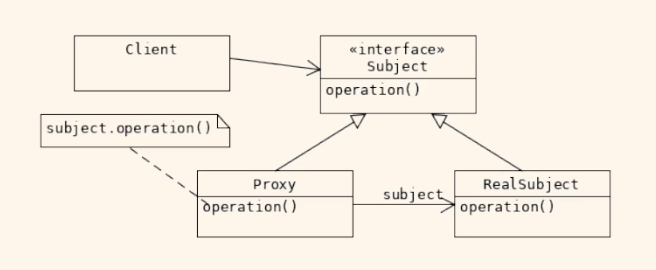
\includegraphics[width=8cm]{ProxyPattern.png}
\end{figure}
\\
Die Vorgehnsweise sieht folgendermaßen aus, nämlich ein User möchte auf einem Objekt eine Methode aufrufen, er ruft die Methode nicht direkt auf dem Objekt auf sondern der Client verwendet ein Interface. Die Implementierung des Interface kann entweder eine abstrakte Klasse sein oder
ein Interface, dass vorgibt welche Methoden definiert werden sollen bzw. zur Verfügung stehen.
Zusätzlich gibt es noch eine Klasse Proxy und RealSubject, auf dem die Operation die von oben vererbet wird ausgeführt wird. Im Remote Proxy Pattern ruft ein Client mit dem Interface auf dem Proxy Objekt einer Operation auf. Diese Proxy Objekt dient als Stellverdrehtung des realen Objekts. Das Proxy Objekt baut nach der Ausführung der Operation
eine Verbindung zu dem wirklichen Objekt auf und über diese Verbindung wird ein Protokoll abgewickelt werden. Bei der Übertragung werden sämtliche Informationen bezüglich des Funktionsaufrufs wie zum Beispiel Eingangsparameter, Ausgabeparameter, Funktionsname mit übertragen. \\\\
Nach der Ausführung wird das Resultat des Objekts anhand des Protokolls zurück zum Proxy Objekt und dann zum Client zurückgesendet. Der Aufruf wirkt wie ein lokaler Aufruf, jedoch funktioniert dies über das verwendete Netzwerk.
Das Sekeleton ist zuständig, die Kommunikation zwischen dem Proxy und dem RealSubject abzuwickeln.\\\\
Problem, die bei der Umsetzung eines Proxy-Patterns aufdrehten können sind vorallem Interoperabilitätsprobleme(Probleme die beim Zusammenspiel zwischen verschiedener Systemen, Techniken oder Organisationen aufdrehten), call-by-refernce, Behandlung von Excpetions, die Transparenz kann nicht gewährleistet werden und die Behandlung von Threads und Prozessen erfolgt nur serverseitig, Client findet den Server nicht, Client stürtzt ab, nachdem senden der Nachricht, Nachricht geht verloren, Server stürzt ab, Antwort geht verloren, Client stürzt ab, bevor diese die Antwort bekommt.
\newpage
\noindent
\begin{description}
    \item[Aufrufvarianten] ~\par
    \begin{itemize}
        \item synchrone Funktionsaufrufe: remote‑invocation send
        \item synchrone Prozeduraufrufe: synchronization send
        \item asynchrone Funktionsaufrufe: no‑wait send
        \item asynchrone Prozeduraufrufe: no‑wait send\\\\
    \end{itemize} 
\end{description}
\textbf{Stream-orientierte Kommunikation}\\
Stream-orientiert Kommunikation, bezeichnet die gleichzeitige Übertragung und Wiedergabe von Video- und Audiodaten über ein Netzwerk.
Dabei werden Streams von Daten versendet, keine Nachrichten, sondern nicht abgeschlossene Informationeneinheiten.
Den Vorgang der Datenübertragung selbst nennt man Streaming und übertragene Programme werden als Livestream oder kurz Stream bezeichnet. Streaming-Media, das über das WWW bzw. HTML angestoßen wurde, wird auch Webradio oder Web-TV genannt. Im Gegensatz zum Herunterladen ist das Ziel beim Streaming nicht, eine Kopie der Medien beim Nutzer anzulegen, sondern die Medien direkt auszugeben, anschließend werden die Daten verworfen.
\\\\
Die Wiedergabe von Programmen über einen Livestream unterscheidet sich meist vom klassischen Rundfunk. Während beim Rundfunk an eine unbestimmte Anzahl Empfänger zugleich gesendet wird, handelt es sich beim Streaming meist jeweils um eine Direktverbindung zwischen dem Server des Senders und dem Client jedes einzelnen Benutzers. Die Verbreitung erfolgt oftmals über Streaming-Portale und internetbasierte Mediatheken.
\cite{communication2}
\newpage
\noindent
\subsection{TCP/IP}



\newpage
\noindent
\section{Implementierung}

\subsection{Projektstruktur}
-----ÜBERARBEITEN-------------\\\\
Das Projekt wurde in 2 wesentlich Verzeichnisse eingeteilt, nämlich in source und documentation. In dem Verzeichniss documentation sind alle Unterlagen der theoretisch Arbeit 
abgelegt worden. Im Verzeichniss source befinden sich alle relevanten Datein der technischen Umsetzung der Aufgabenstellung.
Die drei erwähnten Objekte wurden zu je 3 Module aufgeteilt.
Das heißt die Klassendefinition, Konstruktoren und Methodenprototypen von Santa Claus, Elfen und Rentiere stehen in der jeweiligen h-Datei. Die Methodendefinitionen, der dazugehörigen Klasse,
wurden in der dazugehörigen cpp-Datei kodiert. Zusätzlichen Funktionen die für die Umsetzung des Projekts dringend notwendig waren, wurden in dem Modul utils declariert und definiert.
Da einige Source Code Abschnitte nicht verständlich und nachfollziebar sind, wurden alle Variablen, Funktionen, Klassen, Methoden und sonstiges gut dokumentiert.\\
\newpage
Im unterem Verzeichnissbaum wird die Struktur des Projekts abgebildet
\\
\dirtree{%
.1 documentation\DTcomment{enthält alle Datein der theoretisch Ausarbeitung}.
.2 {Logo.png}.
.2 {SantaClausProblem\_Dokumentation.pdf}.
.2 {SantaClausProblem\_Dokumentation.tex}.
.1 source\DTcomment{enthält alle Datein der praktischen Ausarbeitung}.
.2 build\DTcomment{darin befinden sich alle automatisch generiert Datein}.
.3 {build.ninja}.
.3 {compile\_commands.json}.
.3 {meson\-info}.
.3 {meson\-logs}.
.3 {meson-private}.
.3 {santa\_claus\_problem}.
.3 {santa\_claus\_problem@exe}.
.3 {santa\_problem.json}.
.2 include\DTcomment{darin befinden sich alle h-Dateien}.
.3 {Elves.h}.
.3 {Reindeer.h}.
.3 {SantaClaus.h}.
.3 {utils.h}.
.2 src\DTcomment{darin befinden sich alle cpp-Dateien}.
.3 {Elves.cpp}.
.3 {Reindeer.cpp}.
.3 {SantaClaus.cpp}.
.3 {utils.cpp}.
.3 {main.cpp}.
.2 {meson.build}.
.2 {meson\_options.txt}.
}
\subsection{Klassendiagramme}

\subsection{Source Code Dokumentation}

\subsection{Kommandozeilenparameter}


\subsection{Konsolenausgabe}

\newpage
\noindent
\subsection{Verwendete Bibliotheken}
\subsubsection{CLI11}
CLI11 bietet alle Funktionen, die man von einem leistungsstarken Befehlszeilenparser erwartet, mit einer schönen, minimalen Syntax und ohne 
Abhängigkeiten über C++11 hinaus. Es ist eine header-only, um die Einbindung im Projekte zu 
vereinfachen. CLI11 ist einfach für kleine Projekte zu verwenden, aber leistungsstark genug für komplexe Befehlszeilenprojekte und kann für Frameworks angepasst werden. \\\\
Die Bibliothek wird mit Travis-, AppVeyor-, Azure- und GitHub-Aktionen getestet und vom GooFit-GPU-Anpassungsframework verwendet. 
Es wurde von plumbum.cli für Python inspiriert. CLI11 bietet eine benutzerfreundliche Einführung in diese README-Datei, ein ausführlicheres Tutorial-GitBook sowie eine von Travis generierte API-Dokumentation. 
Weitere Informationen zu aktuellen und früheren Versionen findet man im Changelog oder in den GitHub-Versionen.
\subsubsection{tabulat}
tabulate ist eine reine headeronly-Bibliothek. 
Man legt eine Objekt Table an und kann mittel Table.add\_rows neue Zeilen in der Tabelle hinzufügen.
Die Tabelle kann mittels Table.format() formatieren werden, das ein Format-Objekt zurückgibt. 
Es können damit die Eigenschaften der Tabelle formatieren werden, z. B. Rahmen, Schriftstile, Farben usw.
Auf Zeilen in der Tabelle greift man mitTabelle [row\_index] zu. Dies gibt ein Zeilenobjekt zurück, für das man Row.format() auf ähnliche Weise aufrufen kann, um die Eigenschaften aller Zellen in dieser Zeile zu formatierne.\\
Die Bibliothek wurde verwendet, sodass am Ende des Programmes eine übersichtliche Tabelle ausgegeben werden kann, wie viele Daten in Struktur gebracht wurden.
beinhaltet.
\subsubsection{rang}
rang only hängt von der C++ Standardbibliothek, dem Systemheader unistd.h unter Unix und den Systemheadern windows.h und io.h auf Windows\-basierten Systemen ab. Mit anderen Worten, man benötigen keine Abhängigkeiten von Drittanbietern. Diese Standardbibliothek ermöglich es den
Output der Console zu formatieren. Dabei kann die Schriftart, Farbe und sonstige Eigenschaften bezüglich der Consolenausgabe konfigurieren.
\newpage
\noindent
\subsubsection{json}
In Sprachen wie Python fühlt sich JSON wie ein erstklassiger Datentyp an. 
Die Entwickler haben die ganze Operator-Magie des modernen C++ verwendet, um das gleiche Gefühl in einem c++ Projekt zu erzielen. 
Der gesamter Code besteht aus einer einzelnen Header-Datei json.hpp. Keine Bibliothek, kein Teilprojekt, keine Abhängigkeiten, kein komplexes Build-System. 
Die Klasse ist in Vanilla C++ 11geschrieben. \\\\
Alles in allem ist keine Anpassung der Compiler-Flags oder Projekteinstellungen erforderlich.
Jedes JSON-Objekt hat einen Overhead und einem Aufzählungselement. Die Standardverallgemeinerung verwendet die folgenden C++-Datentypen: std::string für Zeichenfolgen, int64\_t, uint64\_t oder double für Zahlen, std::map für Objekte, std::vector für Arrays und bool für Boolesche Werte. 
json.hpp ist die einzige erforderliche Datei in single\_include/nlohmann, jedoch muss sie im Projekt mit eingebunden werden. \\
Die Libary wurde in diesem Projekt verwendet, um die zusammengefassten Daten des Master-Server abzuspeichern.
\subsubsection{spdlog}
spdlog ist eine sehr effiziente headeronly C++ Protokollierungsbibliothek. Sie bietet auch ebenfalls eine Python-ähnliche Formatierungs-API unter Verwendung der mitgelieferten fmt lib.
spdlog verfolgt den Ansatz "include what you need". Der Source Code sollte die Funktionen enthalten, die tatsächlich benötigt werden.\\\\
Den Programmierer wird eine funktionsreiche Formatierung mit der hervorragenden fmt-Bibliothek geboten.
Im Projekt wird die Libary verwendet, um die Logging Informationen in der Kommandozeile ausgegeben werden kann. Zusätzlich ist es auch möglich
die Logging Daten nicht nur auszugeben, sonder auch direkt in einem Log-File zu schreiben.

\newpage
\noindent
\section{Anwendungsfälle}

\section{Schlusswort}
\newpage
\printbibliography
\end{document}
